% !TEX root = ../main.tex
%\begin{frame}\begin{center}
%\LARGE\textbf{Pipeline}
%\end{center}\end{frame}
\section{Pipeline}
%-------------------------------------------------------------------------------
%-------------------------------------------------------------------------------
\begin{frame}{Tooling}\vspace{0.25cm}
\textbf{respy}\\
\medskip
\begin{tabular}{ll}
GitHub  & \url{OpenSourceEconomics/respy}\\\medskip
Docs    & \url{respy.readthedocs.io}\\
\end{tabular}\bigskip

\textbf{estimagic}\\
\medskip
\begin{tabular}{ll}
GitHub	& \url{OpenSourceEconomics/estimagic}\\\medskip
Docs    & \url{estimagic.readthedocs.io}\\
\end{tabular}

\end{frame}
%-------------------------------------------------------------------------------
%-------------------------------------------------------------------------------
\begin{frame}{Workflow}
	\begin{figure}
	   \lstset{basicstyle=\scriptsize\ttfamily, language=python, morekeywords={as}, ndkeywords={=}, ndkeywordstyle=\color{blue}, keywordstyle=\color{red}, commentstyle=\color{darkgrey}, emph={get_example_model, get_crit_func, get_simulate_func}, emphstyle=\color{violet}}
	   \lstinputlisting{../material/workflow.py}
   \end{figure}
\end{frame}
%-------------------------------------------------------------------------------
%-------------------------------------------------------------------------------
\begin{frame}{Model parameterization}

	\begin{figure}[h!]\centering
	\scalebox{0.60}{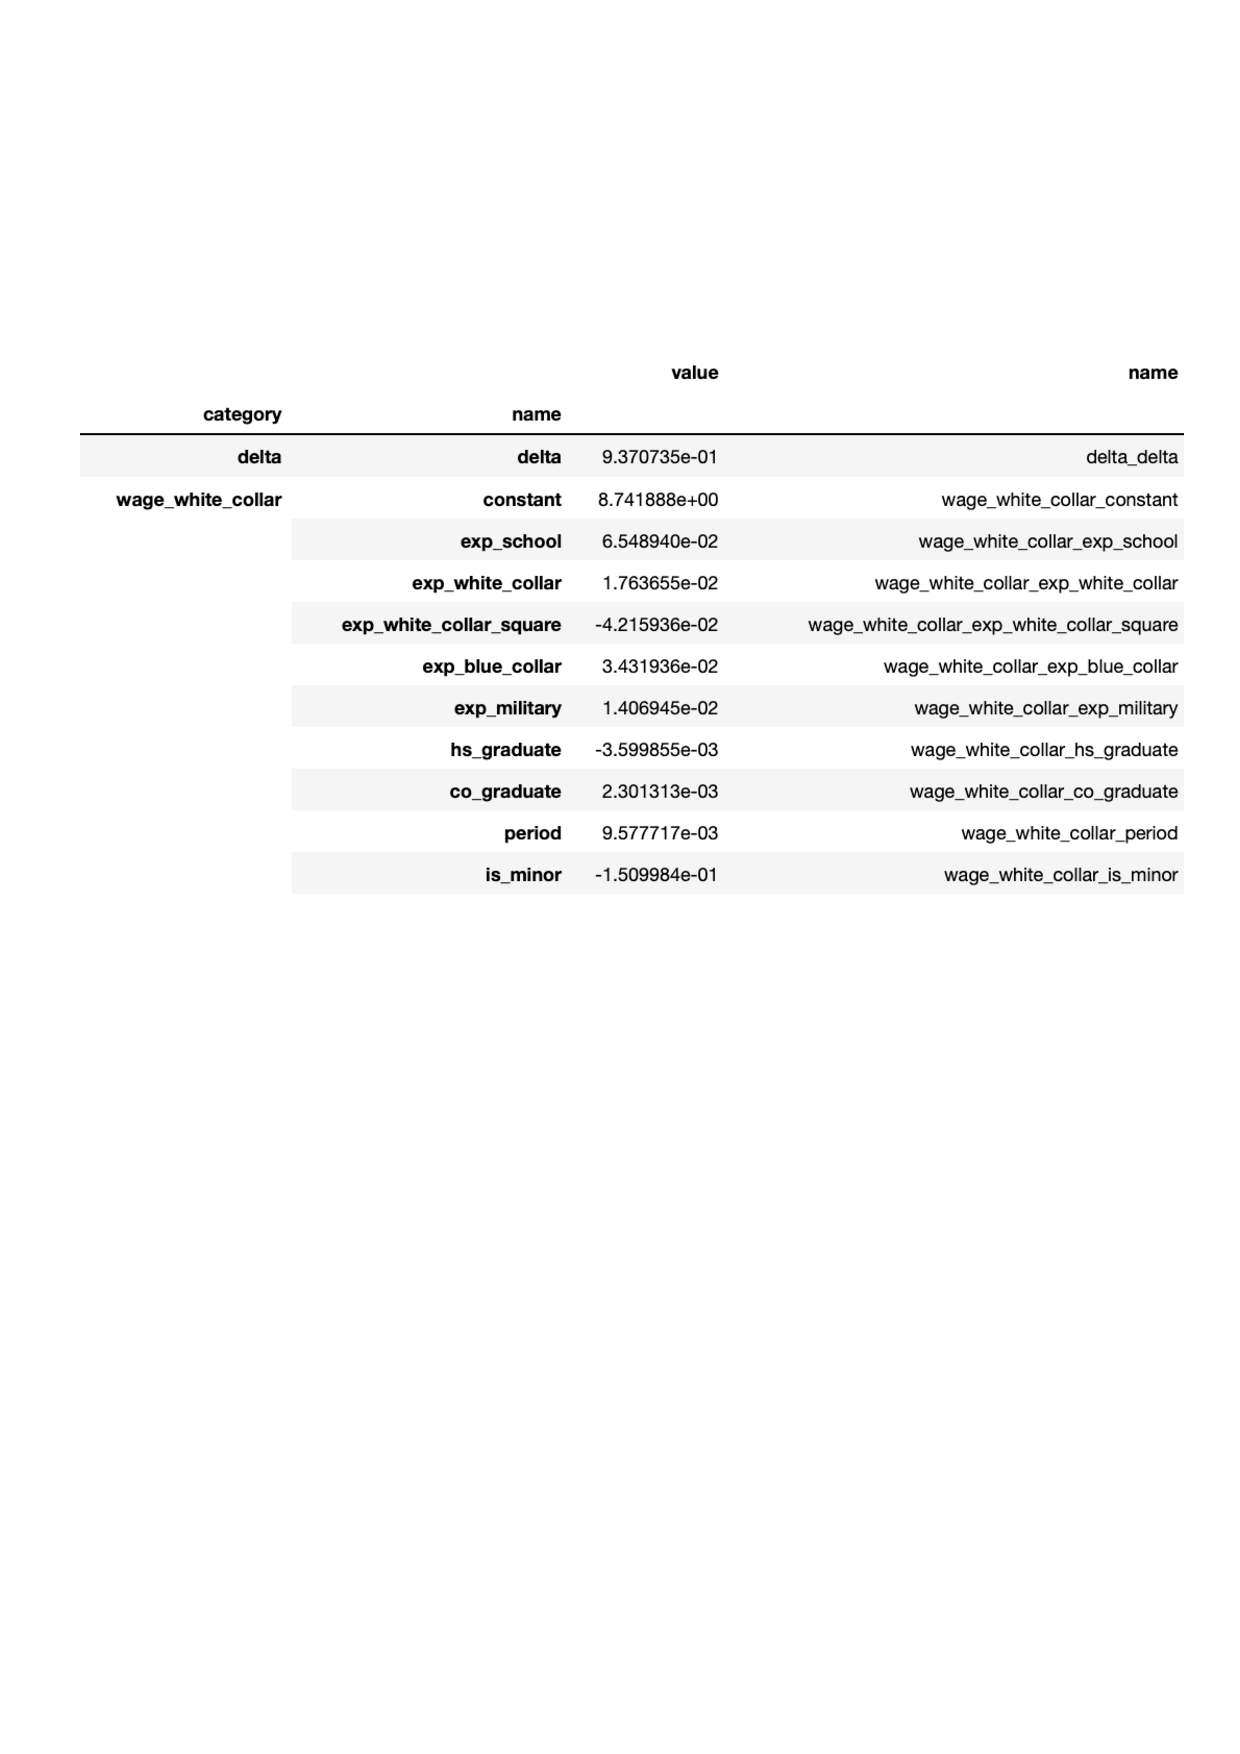
\includegraphics{crop-params}}
	\end{figure}

\end{frame}
%-------------------------------------------------------------------------------
%-------------------------------------------------------------------------------
\begin{frame}{Options}

	\begin{figure}[h!]\centering
	\scalebox{0.60}{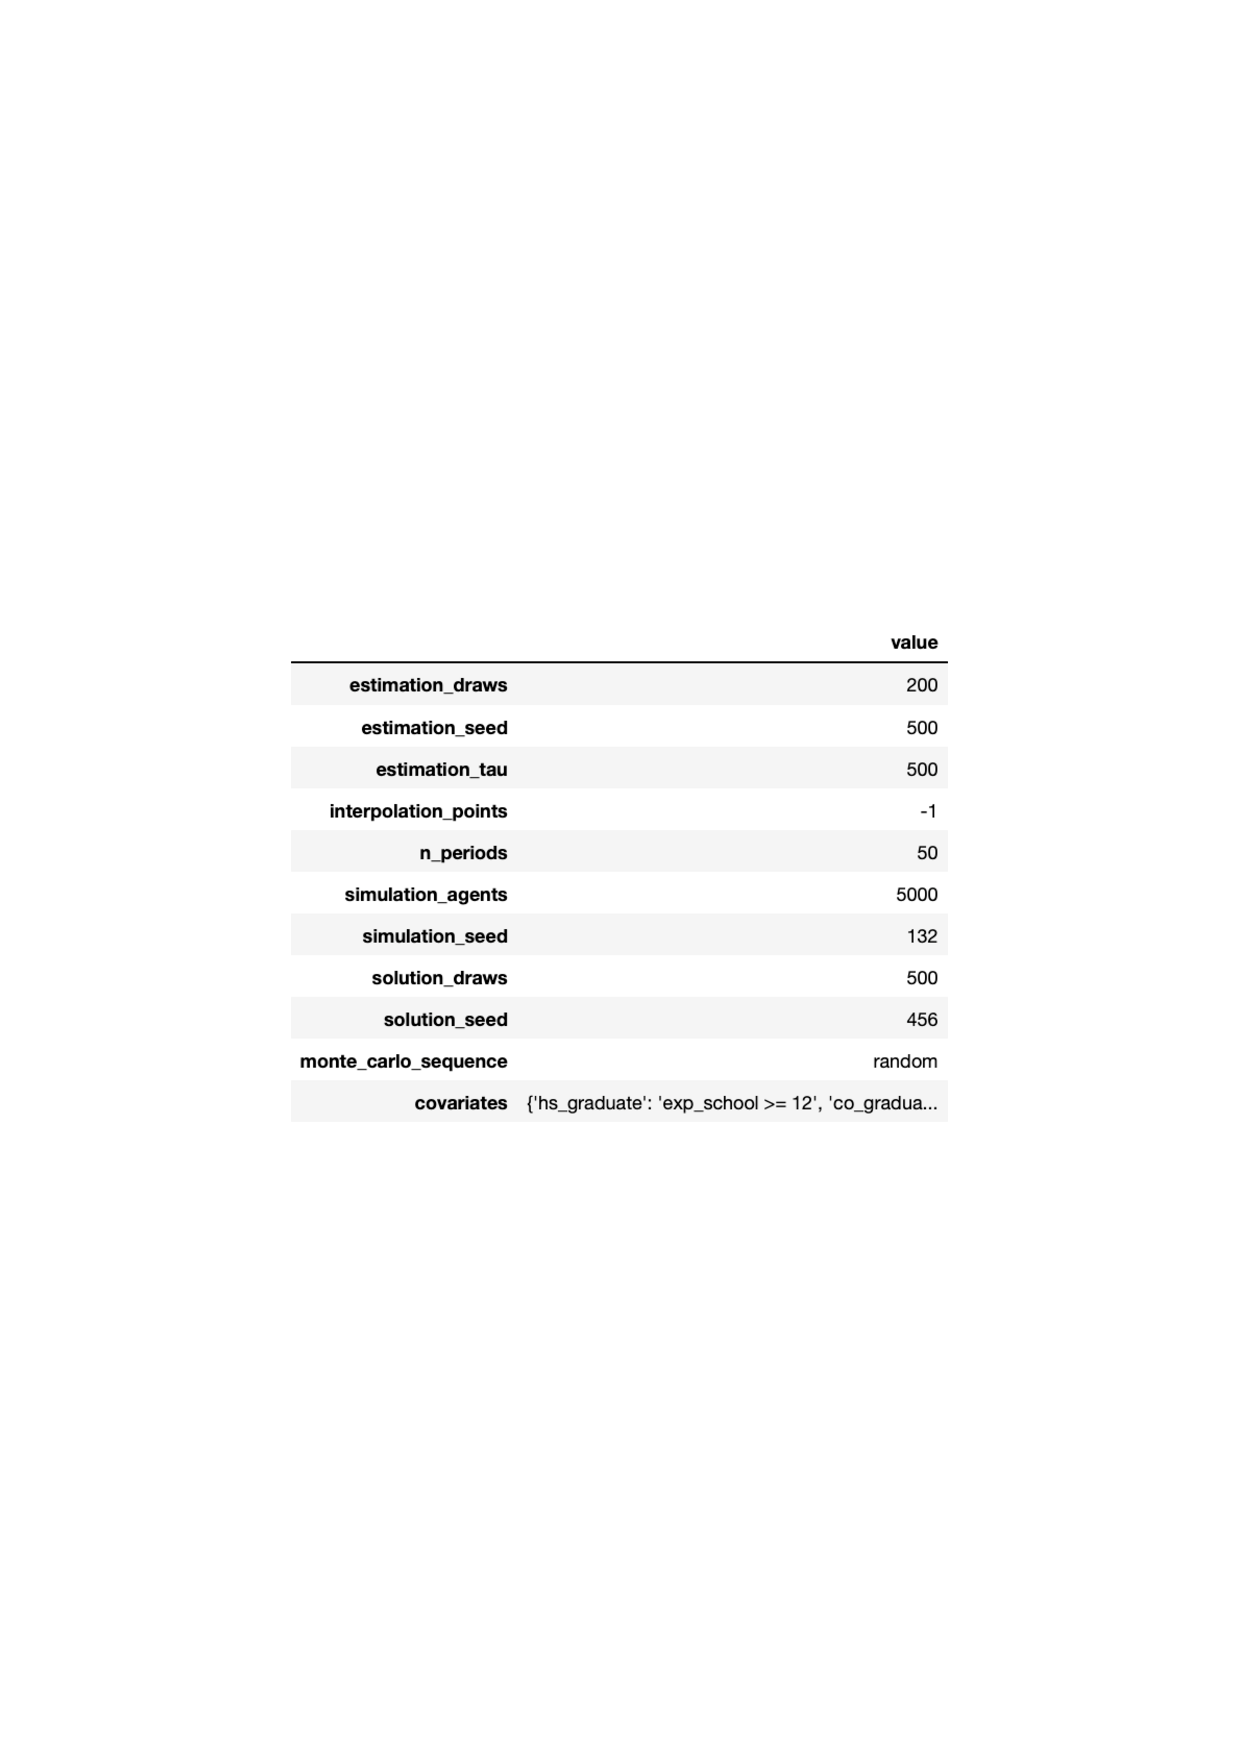
\includegraphics{crop-options}}
	\caption{Model options}\label{Model options}
\end{figure}

\end{frame}
%-------------------------------------------------------------------------------
%-------------------------------------------------------------------------------
